\documentclass[10pt,a4paper]{article}
\usepackage[T1]{fontenc}
\usepackage[utf8]{inputenc}
\usepackage{lmodern}
\renewcommand{\familydefault}{\sfdefault}
\usepackage[a4paper,margin=1.9cm,top=1.7cm,bottom=1.8cm]{geometry}
\usepackage{microtype}
\usepackage{xcolor}
\usepackage{graphicx}
\usepackage[font=small,labelfont=bf,skip=3pt]{caption}
\usepackage{subcaption}
\usepackage{float}
\usepackage{booktabs}
\usepackage{tabularx}
\usepackage{enumitem}
\usepackage{titlesec}
\usepackage{fancyhdr}
\usepackage{tikz}
\usetikzlibrary{positioning,fit,arrows.meta,backgrounds,calc}
\usepackage[hidelinks]{hyperref}

\definecolor{ink}{HTML}{1F2937}
\definecolor{accent}{HTML}{2563EB}
\definecolor{sched}{HTML}{DBEAFE}
\definecolor{trips}{HTML}{DCFCE7}
\definecolor{azure}{HTML}{F1F5F9}
\definecolor{warn}{HTML}{B91C1C}
\definecolor{muted}{HTML}{6B7280}

\titleformat{\section}{\large\bfseries\color{ink}}{\thesection}{0.6em}{}
\titleformat{\subsection}{\normalsize\bfseries\color{ink}}{\thesubsection}{0.5em}{}
\titlespacing*{\section}{0pt}{9pt}{4pt}
\titlespacing*{\subsection}{0pt}{6pt}{2pt}
\setlist{nosep,leftmargin=1.2em}
\setlength{\parindent}{0pt}
\setlength{\parskip}{3.5pt}
\pagestyle{fancy}\fancyhf{}
\renewcommand{\headrulewidth}{0pt}
\fancyfoot[L]{\footnotesize\color{muted}TripSync --- Individual Assignment 2}
\fancyfoot[R]{\footnotesize\color{muted}\thepage}

\newcommand{\code}[1]{\texttt{#1}}

\tikzset{
  box/.style={draw=ink!70,rounded corners=2pt,align=center,font=\footnotesize,inner sep=3pt,fill=white},
  db/.style={draw=ink!70,cylinder,shape border rotate=90,aspect=0.18,align=center,font=\footnotesize,inner sep=2pt,fill=white,minimum width=2.3cm},
  grp/.style={draw=ink!40,rounded corners=4pt,inner sep=5pt},
  lbl/.style={font=\scriptsize\color{muted},align=center,fill=white,inner sep=1pt},
  arr/.style={-{Stealth[length=5pt]},draw=ink!80},
  call/.style={-{Stealth[length=5pt]},draw=accent,thick},
}
\usetikzlibrary{shapes.geometric,shapes.multipart}

\begin{document}

\begin{center}
{\LARGE\bfseries\color{ink} TripSync: split, shipped and operated}\\[3pt]
{\normalsize Software Development and DevOps --- Individual Assignment 2}\\[2pt]
{\small Alejandro Zapata (\code{azapata.ieu2024}) \quad\textbullet\quad 22 November 2026}\\[4pt]
{\small Live: \href{https://azapataieu2024ui.z28.web.core.windows.net}{\code{https://azapataieu2024ui.z28.web.core.windows.net}}}\\[1pt]
{\small Repository: \href{https://github.com/TheAleZap/devops_assignment_2}{\code{https://github.com/TheAleZap/devops\_assignment\_2}} (graded commit: tag \code{submission})}
\end{center}

\section{Goals, stakeholders and process}

TripSync helps a group of friends agree on \emph{when} to travel (Scheduling) and then organise the trip (Trips).
Assignment~1 was one process with one SQLite file; this iteration turns it into something a real group could rely on.

\textbf{Stakeholders.} The \emph{trip organiser}, who today chases dates in a group chat and needs the plan to be reliable;
the \emph{group members}, who open a link once or twice and must not hit a blank page or lose what they entered;
the \emph{course professors}, who grade the deployed system with Reader access to my resource group;
and \emph{me as the developer and operator}, who pays (in credit) for whatever runs and has to fix what breaks.

\textbf{SMART goals} (product outcomes, all due by 22 Nov 2026):
\begin{enumerate}
  \item A group can open the public URL, mark availability, see the best dates and confirm them on a trip, end to end on Azure. \emph{Met} (evidence 09, 10).
  \item Confirming dates never leaves a trip half-updated: if Scheduling is down, the organiser sees a clear message within 10\,s and the trip is unchanged, in 100\% of the integration-test runs. \emph{Met} (§5.2).
  \item A schema change reaches production without losing data: migration 002 is deployed by the pipeline and trip \#1 keeps all its members, dates, claims and done flags. \emph{Met} (§5.1).
  \item Every merged change reaches users in under 10 minutes with no manual step, and a change that breaks the API contract never reaches them. \emph{Met}: CD takes 4--6 min; the contract gate blocked a stale contract (§5.3).
  \item An idle week costs (close to) nothing: everything scales to zero or pauses. \emph{Met} by design (ADR-8); credit use stayed negligible.
\end{enumerate}

\textbf{Process.} I kept the iterative, incremental model of Assignment 1, but with a stricter loop: one small increment per branch,
a pull request so CI runs before anything reaches \code{main}, a merge commit, and an automatic deploy. Each day had one theme
(split, data, compose, CI, Azure, migration, polish), and decisions were written as ADRs on the day they were made (ADR 6--10 span five dates).

\section{Architecture: before and after}

\begin{figure}[H]
\centering
\begin{subfigure}[t]{0.30\textwidth}\centering
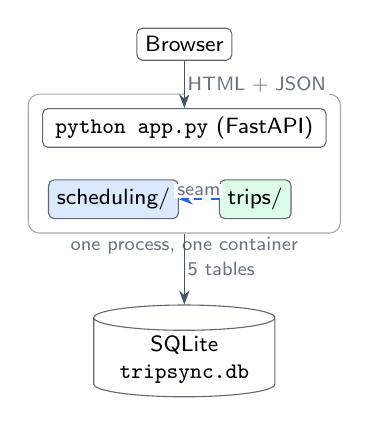
\begin{tikzpicture}[node distance=5mm]
  \node[box] (br) {Browser};
  \node[box,below=6mm of br,minimum width=3.6cm] (app) {\code{python app.py} (FastAPI)};
  \node[box,below=4mm of app,xshift=-9mm,fill=sched] (s) {scheduling/};
  \node[box,below=4mm of app,xshift=9mm,fill=trips] (t) {trips/};
  \node[grp,fit=(app)(s)(t),label={[lbl]below:one process, one container}] (proc) {};
  \node[db,below=9mm of proc] (sq) {SQLite\\\code{tripsync.db}};
  \draw[arr] (br) -- node[lbl,right]{HTML + JSON} (app);
  \draw[call,dashed] (t) -- node[lbl,above]{seam} (s);
  \draw[arr] (proc) -- node[lbl,right]{5 tables} (sq);
\end{tikzpicture}
\caption{Assignment 1: monolith}
\end{subfigure}\hfill
\begin{subfigure}[t]{0.68\textwidth}\centering
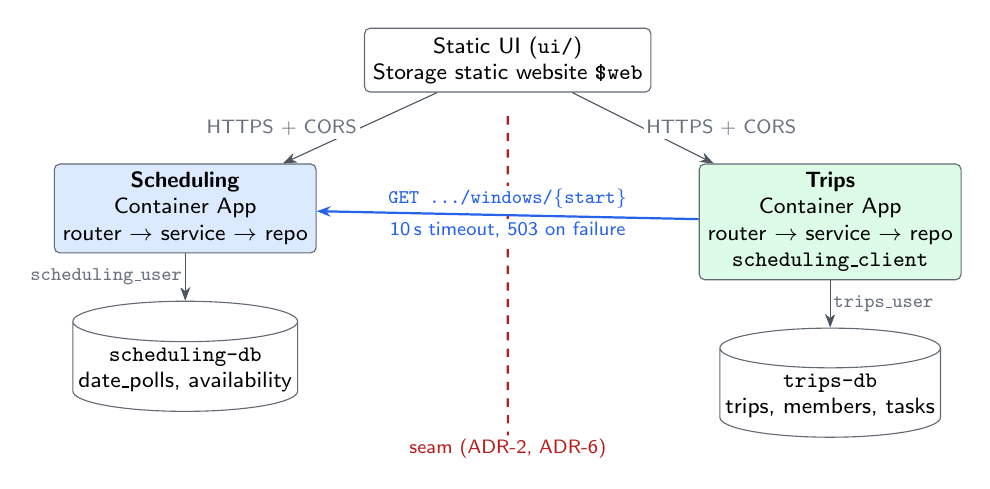
\begin{tikzpicture}
  \node[box] (ui) {Static UI (\code{ui/})\\Storage static website \code{\$web}};
  \node[box,fill=sched,below left=9mm and 6mm of ui,minimum width=2.8cm] (s) {\textbf{Scheduling}\\Container App\\router $\to$ service $\to$ repo};
  \node[box,fill=trips,below right=9mm and 6mm of ui,minimum width=2.8cm] (t) {\textbf{Trips}\\Container App\\router $\to$ service $\to$ repo\\\code{scheduling\_client}};
  \node[db,below=6mm of s] (sd) {\code{scheduling-db}\\date\_polls, availability};
  \node[db,below=6mm of t] (td) {\code{trips-db}\\trips, members, tasks};
  \draw[arr] (ui) -- node[lbl,left]{HTTPS + CORS} (s);
  \draw[arr] (ui) -- node[lbl,right]{HTTPS + CORS} (t);
  \draw[call] (t) -- node[lbl,above=1pt,text=accent]{\code{GET .../windows/\{start\}}} node[lbl,below=1pt,text=accent]{10\,s timeout, 503 on failure} (s);
  \draw[arr] (s) -- node[lbl,left]{\code{scheduling\_user}} (sd);
  \draw[arr] (t) -- node[lbl,right]{\code{trips\_user}} (td);
  \begin{scope}[on background layer]
  \draw[warn,dashed,thick] ($(s.north east)!0.5!(t.north west)+(0,0.6)$) -- ($(sd.south east)!0.5!(td.south west)+(0,-0.15)$) node[lbl,below,text=warn]{seam (ADR-2, ADR-6)};
  \end{scope}
\end{tikzpicture}
\caption{Assignment 2: two services, two databases}
\end{subfigure}
\caption{The seam did not move. The in-process call \code{describe\_window()} became one HTTP call; no table crossed it.}
\end{figure}

The only flow that crosses the seam is \emph{confirm dates}, and it stays server side so Trips never stores attendance data
supplied by the browser (ADR-6). Trips keeps only the poll's ID (a plain integer, ADR-3), the confirmed dates, and nothing else
from Scheduling. Each service logs one line per request and exposes \code{GET /health}, which reports its own database and the deployed commit SHA.

\section{Databases (one per service, matching the migrations)}

Splitting the database cost no database-level integrity, because \code{trips.date\_poll\_id} was already a plain ID in Assignment~1.
What remains is a possible dangling poll ID if Scheduling ever deletes a poll; the app never deletes polls, and confirming dates
always re-reads the window from Scheduling, so a missing poll is reported as 404 instead of being trusted (ADR-7).

\begin{figure}[H]
\centering
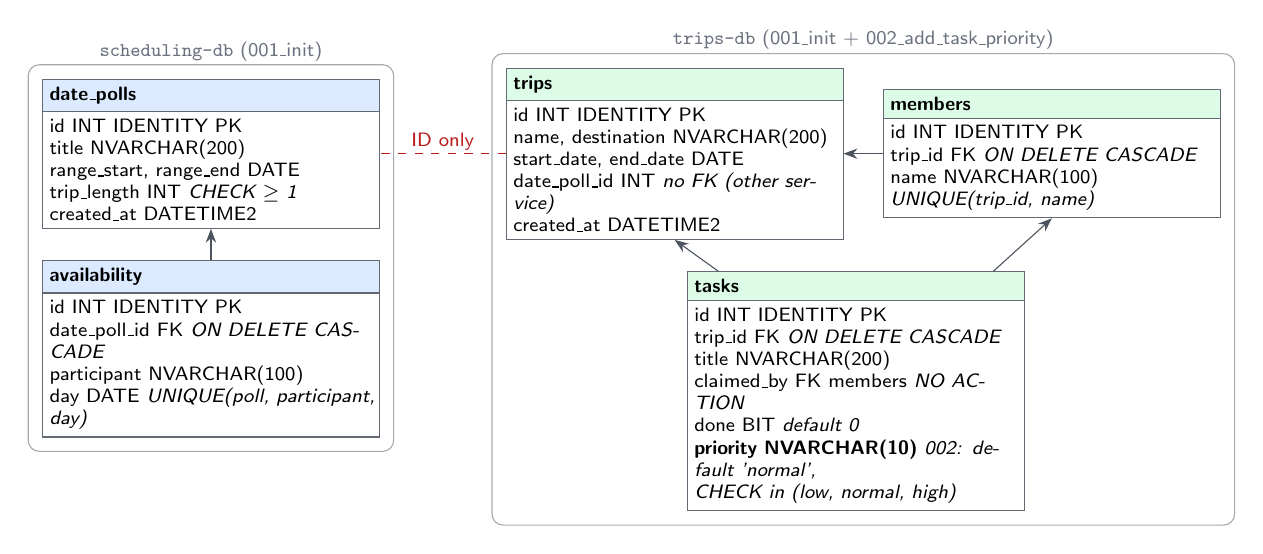
\begin{tikzpicture}[
  tbl/.style={draw=ink!70,rectangle split,rectangle split parts=2,rectangle split part fill={#1,white},align=left,font=\scriptsize,inner sep=2.5pt,text width=4.1cm},
]
\node[tbl=sched] (dp) {\textbf{date\_polls}\nodepart{two}id INT IDENTITY PK\\title NVARCHAR(200)\\range\_start, range\_end DATE\\trip\_length INT \textit{CHECK $\ge$ 1}\\created\_at DATETIME2};
\node[tbl=sched,below=4mm of dp] (av) {\textbf{availability}\nodepart{two}id INT IDENTITY PK\\date\_poll\_id FK \textit{ON DELETE CASCADE}\\participant NVARCHAR(100)\\day DATE \textit{UNIQUE(poll, participant, day)}};
\draw[arr] (av.north) -- (dp.south);
\node[grp,fit=(dp)(av),label={[lbl]above:\code{scheduling-db} (001\_init)}] {};

\node[tbl=trips,right=1.6cm of dp] (tr) {\textbf{trips}\nodepart{two}id INT IDENTITY PK\\name, destination NVARCHAR(200)\\start\_date, end\_date DATE\\date\_poll\_id INT \textit{no FK (other service)}\\created\_at DATETIME2};
\node[tbl=trips,right=5mm of tr] (me) {\textbf{members}\nodepart{two}id INT IDENTITY PK\\trip\_id FK \textit{ON DELETE CASCADE}\\name NVARCHAR(100)\\\textit{UNIQUE(trip\_id, name)}};
\node[tbl=trips,below=4mm of tr,xshift=2.3cm] (ta) {\textbf{tasks}\nodepart{two}id INT IDENTITY PK\\trip\_id FK \textit{ON DELETE CASCADE}\\title NVARCHAR(200)\\claimed\_by FK members \textit{NO ACTION}\\done BIT \textit{default 0}\\\textbf{priority NVARCHAR(10)} \textit{002: default 'normal',}\\\textit{CHECK in (low, normal, high)}};
\draw[arr] (me.west) -- (tr.east);
\draw[arr] (ta.north west) ++(0.4,0) -- (tr.south);
\draw[arr] (ta.north east) ++(-0.4,0) -- (me.south);
\node[grp,fit=(tr)(me)(ta),label={[lbl]above:\code{trips-db} (001\_init + 002\_add\_task\_priority)}] {};
\draw[warn,dashed] (tr.west) -- node[lbl,above,text=warn]{ID only} (dp.east);
\end{tikzpicture}
\caption{Each database also has \code{schema\_migrations(version, applied\_at)}. The dashed line is a plain integer, not a foreign key.}
\end{figure}


\section{Deployment}

\begin{figure}[H]
\centering
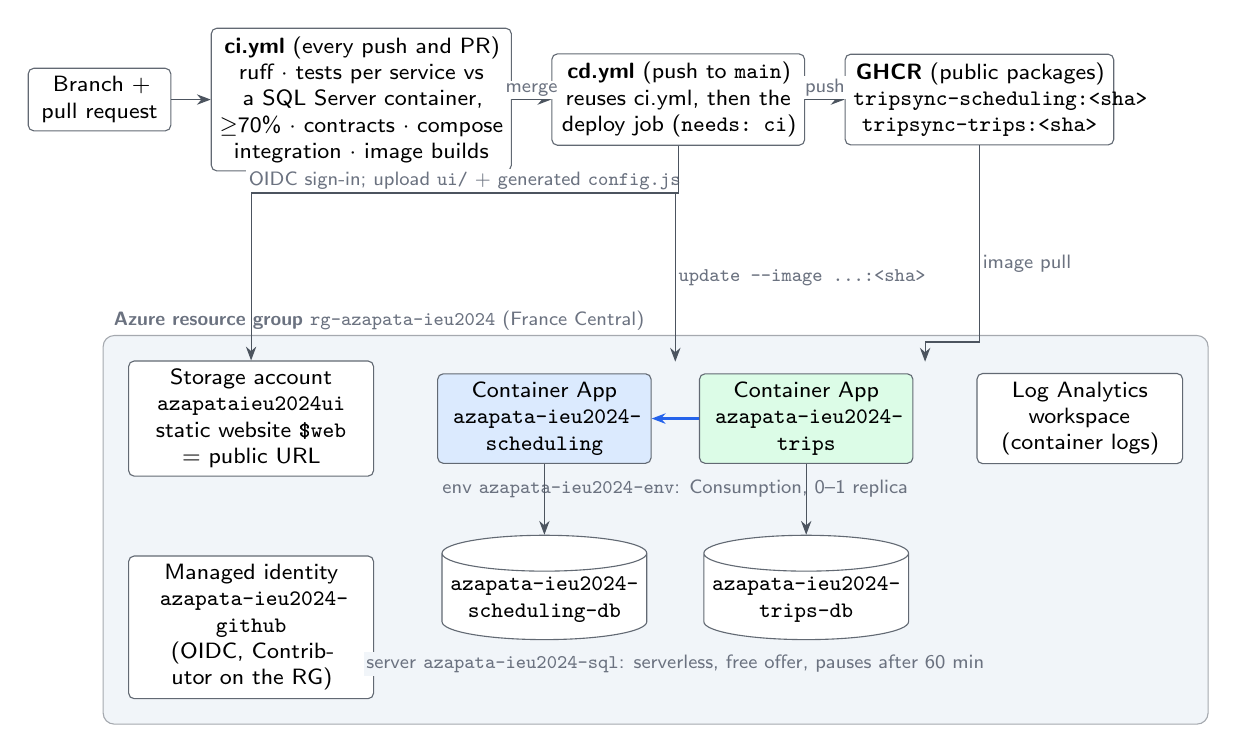
\begin{tikzpicture}[node distance=5mm]
  \node[box,text width=1.6cm] (pr) {Branch +\\pull request};
  \node[box,right=of pr,text width=3.6cm] (ci) {\textbf{ci.yml} (every push and PR)\\ruff $\cdot$ tests per service vs a SQL Server container, $\ge$70\% $\cdot$ contracts $\cdot$ compose integration $\cdot$ image builds};
  \node[box,right=of ci,text width=3.0cm] (cd) {\textbf{cd.yml} (push to \code{main})\\reuses ci.yml, then the deploy job (\code{needs: ci})};
  \node[box,right=of cd,text width=3.2cm] (gh) {\textbf{GHCR} (public packages)\\\code{tripsync-scheduling:<sha>}\\\code{tripsync-trips:<sha>}};
  \draw[arr] (pr) -- (ci);
  \draw[arr] (ci) -- node[lbl,above]{merge} (cd);
  \draw[arr] (cd) -- node[lbl,above]{push} (gh);

  % Azure resource group
  \node[box,below=24mm of ci,xshift=-14mm,text width=2.9cm] (st) {Storage account\\\code{azapataieu2024ui}\\static website \code{\$web} = public URL};
  \node[box,fill=sched,right=8mm of st,text width=2.5cm] (cs) {Container App\\\code{azapata-ieu2024-}\\\code{scheduling}};
  \node[box,fill=trips,right=6mm of cs,text width=2.5cm] (ct) {Container App\\\code{azapata-ieu2024-}\\\code{trips}};
  \node[box,right=8mm of ct,text width=2.4cm] (la) {Log Analytics workspace\\(container logs)};
  \node[db,below=9mm of cs,minimum width=2.6cm] (dsd) {\code{azapata-ieu2024-}\\\code{scheduling-db}};
  \node[db,below=9mm of ct,minimum width=2.6cm] (dtd) {\code{azapata-ieu2024-}\\\code{trips-db}};
  \node[box,below=10mm of st,text width=2.9cm] (mi) {Managed identity\\\code{azapata-ieu2024-}\\\code{github}\\(OIDC, Contributor on the RG)};
  \begin{scope}[on background layer]
    \node[grp,fill=white,fit=(cs)(ct),inner sep=4pt] (env) {};
    \node[grp,fill=white,fit=(dsd)(dtd),inner sep=4pt] (sql) {};
    \node[grp,fill=azure,fit=(st)(env)(la)(sql)(mi),inner sep=9pt] (rg) {};
  \end{scope}
  \node[lbl,anchor=south west,fill=none] at ($(rg.north west)+(0.1,0.02)$) {\textbf{Azure resource group \code{rg-azapata-ieu2024}} (France Central)};
  \node[lbl,fill=azure,anchor=north] at ($(env.south)+(0,-0.02)$) {env \code{azapata-ieu2024-env}: Consumption, 0--1 replica};
  \node[lbl,fill=azure,anchor=north] at (sql.south) {server \code{azapata-ieu2024-sql}: serverless, free offer, pauses after 60 min};
  \draw[arr] (cs) -- (dsd); \draw[arr] (ct) -- (dtd);
  \draw[call] (ct) -- (cs);
  \draw[arr] (gh.south) |- node[lbl,pos=0.3,right]{image pull} ($(env.north east)+(0,0.25)$) -- (env.north east);
  \draw[arr] (cd.south) -- ++(0,-6mm) -| node[lbl,pos=0.25,above]{OIDC sign-in; upload \code{ui/} + generated \code{config.js}} (st.north);
  \draw[arr] (cd.south) -- ++(0,-6mm) -| node[lbl,pos=0.75,right]{\code{update --image ...:<sha>}} (env.north);
\end{tikzpicture}
\caption{GitHub $\to$ Actions $\to$ GHCR $\to$ Azure. After the one-off setup (in the README), nothing is changed by hand: CD signs in with OIDC (no Azure password stored), stores each \code{DATABASE\_URL} as a Container Apps secret, deploys the SHA-tagged images, publishes the UI, and only passes when both \code{/health} endpoints report the new SHA (it waits up to 6 min, to cover a database resuming from pause).}
\end{figure}

\section{Evidence}

\subsection{Migration on Azure (migration 002, deployed by CD run \href{https://github.com/TheAleZap/devops_assignment_2/actions/runs/44907062326}{44907062326})}

\code{002\_add\_task\_priority.sql} adds \code{priority NVARCHAR(10) NOT NULL DEFAULT 'normal'} with a \code{CHECK} to \code{tasks},
which already held trip \#1's three tasks. It is expand-only, so the previous revision (which inserts tasks without the column)
kept working during the rollout; a test (\code{test\_task\_inserted\_without\_priority\_gets\_normal}) proves that case.

\begin{figure}[H]
\centering
\begin{subfigure}[t]{0.31\textwidth}\centering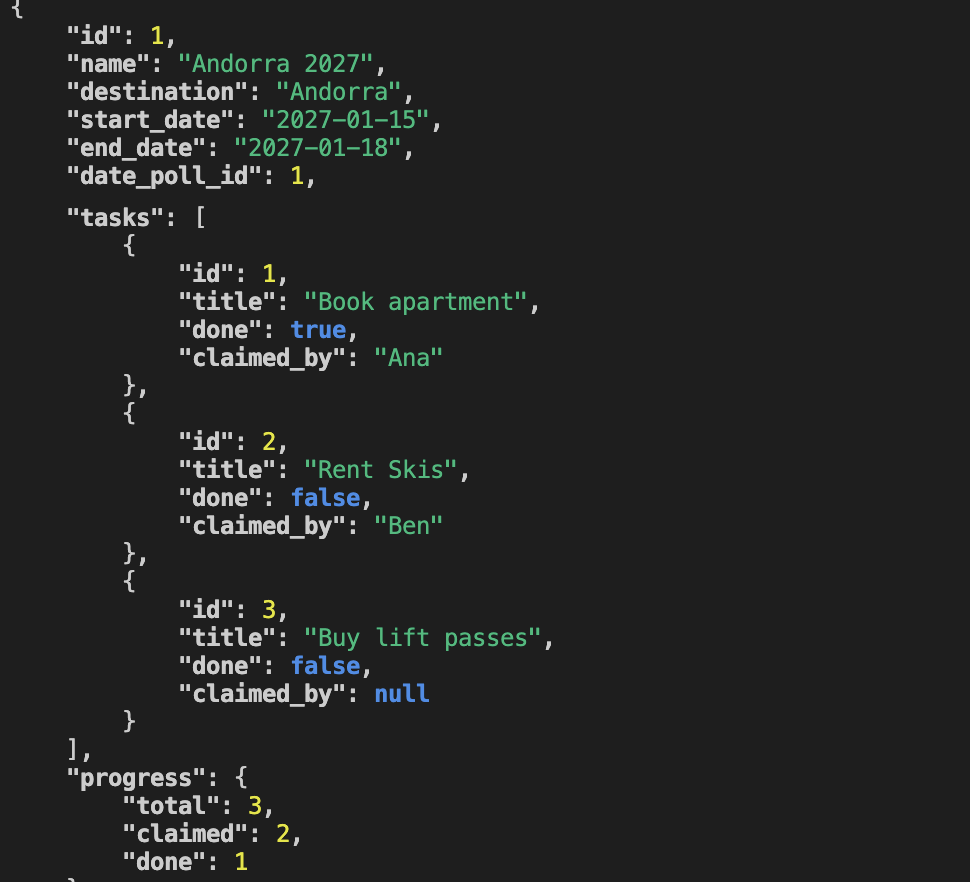
\includegraphics[width=\linewidth]{figures/before-crop.png}\caption{Before the deploy: no \code{priority} field}\end{subfigure}\hspace{0.06\textwidth}
\begin{subfigure}[t]{0.31\textwidth}\centering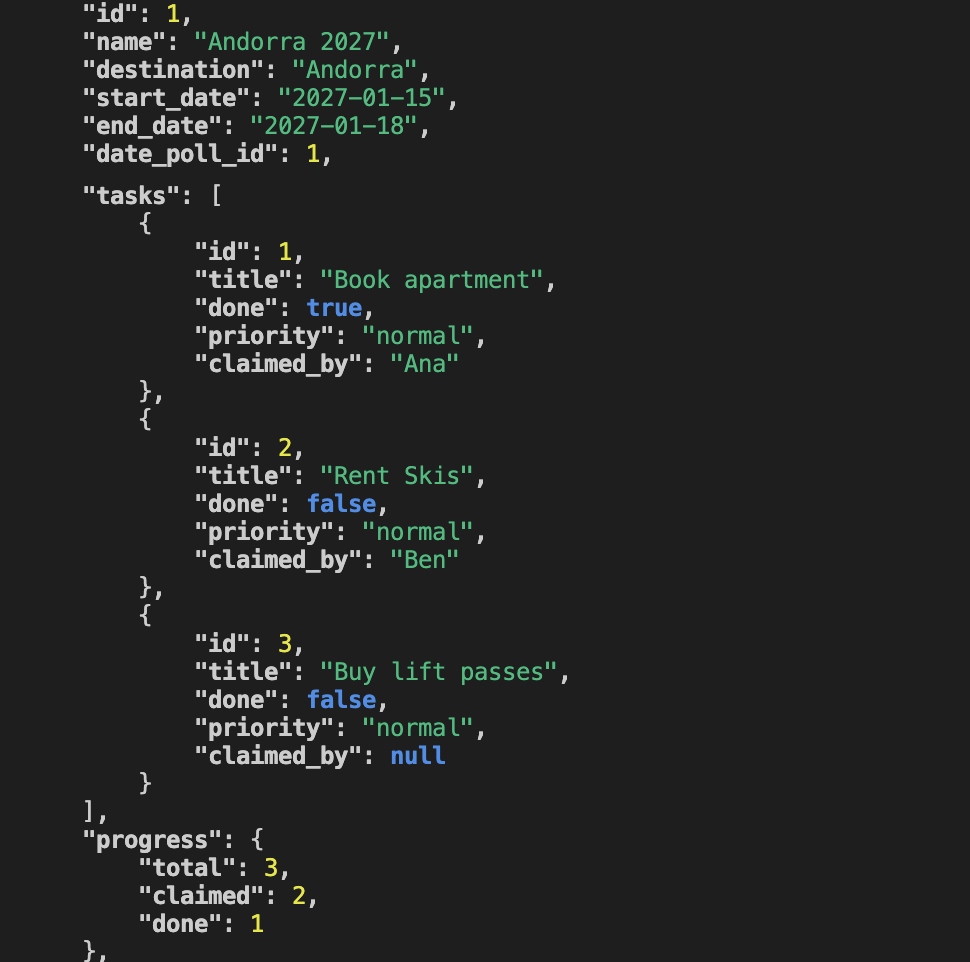
\includegraphics[width=\linewidth]{figures/after-crop.png}\caption{After: same data, plus \code{"priority": "normal"}}\end{subfigure}\\[3pt]
\begin{subfigure}[t]{0.72\textwidth}\centering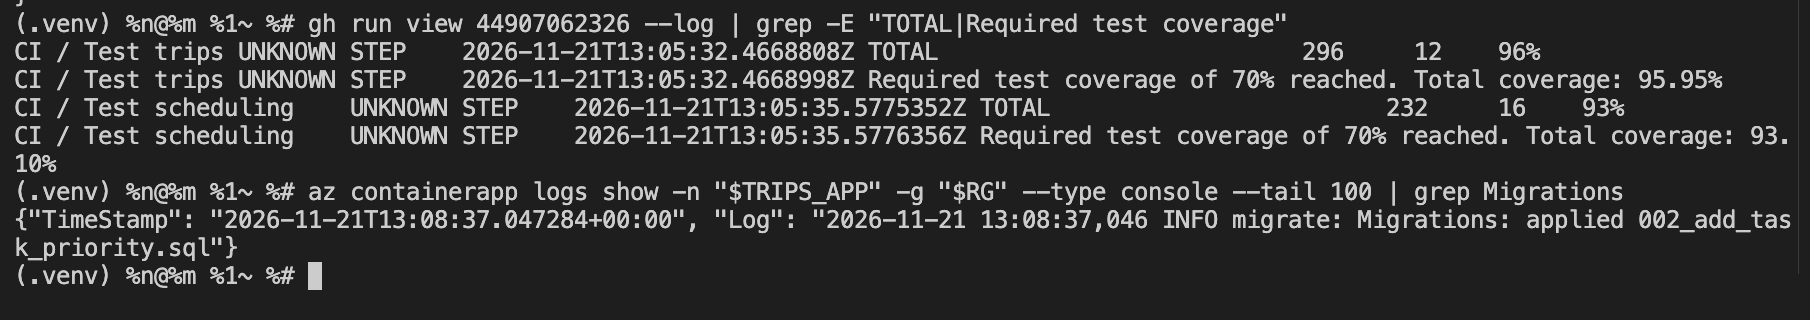
\includegraphics[width=\linewidth]{figures/14-migration-002-log.png}\caption{Startup log on Azure: \code{Migrations: applied 002\_add\_task\_priority.sql} (13:08:37 UTC)}\end{subfigure}
\caption{Trip \#1 on Azure before and after: dates (15--18 Jan 2027, poll 1), members, claims, done flags and progress 3/2/1 are identical; only the new column appears. Members (Ana, Ben, Carla) are cropped out and also unchanged (full screenshots 13 and 15 in the repository).}
\end{figure}

\subsection{Partial failure}

\begin{figure}[H]
\centering
\begin{minipage}[c]{0.36\textwidth}\centering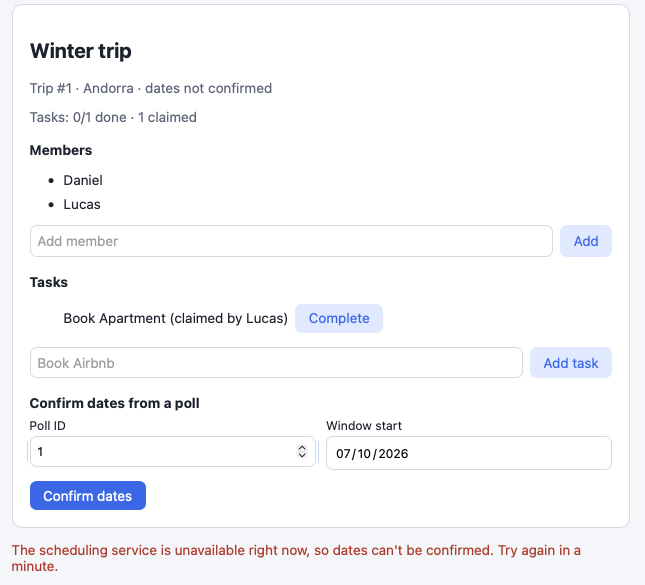
\includegraphics[width=\linewidth]{figures/partial-failure.png}\end{minipage}\hfill
\begin{minipage}[c]{0.60\textwidth}
\small With Scheduling stopped (\code{docker compose stop scheduling}), Trips still loads trips, adds members and tasks, and claims
and completes them. Only \emph{Confirm dates} fails, by design: \code{scheduling\_client} raises \code{SchedulingUnavailable}
on a connection error, a timeout or a 5xx, the router returns \textbf{503} with
\emph{``The scheduling service is unavailable right now, so dates can't be confirmed. Try again in a minute.''},
and \code{set\_trip\_dates} is never called, so the trip is unchanged. An unknown poll gives 404 and a window outside the poll 400.
The Scheduling tab shows a clear ``can't be reached'' message instead of a blank page. On Azure, the UI also retries Azure's own
cold-start 503 page and shows ``starting up'' (ADR-8). The CI integration test stops Scheduling and asserts this 503 on every run.
\end{minipage}
\caption{What a user sees when the other service is down (local compose, evidence 01--04).}
\end{figure}

\subsection{Pipeline}

\begin{itemize}
  \item \textbf{Successful CD run on \code{main}}: \href{https://github.com/TheAleZap/devops_assignment_2/actions/runs/44907062326}{run 44907062326} (migration 002: CI, SHA-tagged images, deploy, health check on the SHA), and the first deploy, \code{3e865f0} (evidence 11).
  \item \textbf{Failed run that was fixed}: \href{https://github.com/TheAleZap/devops_assignment_2/actions/runs/45013261916}{run 45013261916} $\to$ fixed in \href{https://github.com/TheAleZap/devops_assignment_2/actions/runs/45013755471}{run 45013755471} (PR \#12).
  \emph{This failure was deliberate.} No run had failed by accident during the week (I ran ruff, pytest and \code{export\_openapi.py} locally before every push), so I tested the contract gate on purpose while adding a real feature, an endpoint to change a task's priority.
  \textbf{Cause:} the new \code{PUT /api/trips/\{trip\_id\}/tasks/\{task\_id\}/priority} was committed without regenerating \code{openapi.json}; the \emph{contracts} job regenerated the document from the code, diffed it with the committed file, found the missing operation and exited 1. Lint, tests and the integration test passed, and both image builds were \emph{skipped} because they need every gate, so nothing could reach GHCR or Azure.
  \textbf{Fix:} regenerate and commit \code{openapi.json}; all 14 checks passed and the PR was merged and deployed.
\end{itemize}
\begin{figure}[H]
\centering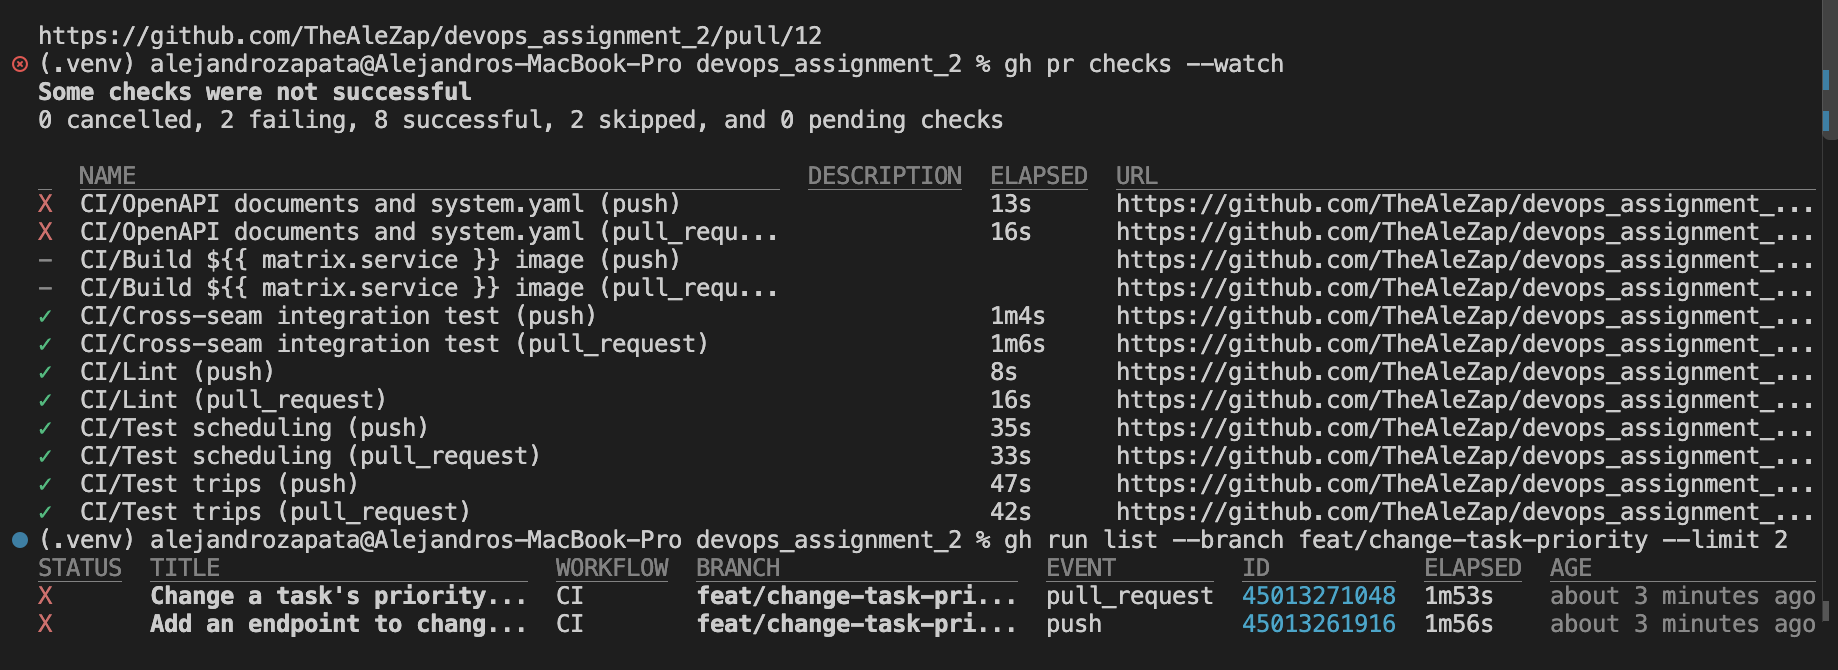
\includegraphics[width=0.72\textwidth]{figures/16-ci-contract-gate-failed.png}
\caption{The deliberate failure: only the contract job fails, and the builds are skipped.}
\end{figure}

\subsection{README}
The README covers running the whole system with \code{docker compose up --build}, running one service (Trips has no
\code{depends\_on} on Scheduling), running the tests and coverage against a throwaway database (CI: Scheduling 93.10\%, Trips 95.95\%),
how CI/CD deploys, the initial Azure setup step by step, and the live URL.

\section{Plan versus actual}

\begin{tabularx}{\textwidth}{@{}l l X r@{}}
\toprule
\textbf{Day} & \textbf{Planned} & \textbf{What actually happened} & \textbf{Commits}\\
\midrule
Mon 16 & Fork A1, split into two services & Done (ADR-6). iCloud returned \code{mmap failed} mid-push and later half-overwrote the working tree; recovered with \code{git restore} and \code{git fsck}. & 4\\
Tue 17 & SQL Server, migrations, Docker & Done (ADR-7). SQL Server rejected \code{ON DELETE SET NULL} on \code{claimed\_by} (two cascade paths), so it became \code{NO ACTION}; a changed \code{.env} broke the DB password until I recreated the container. & 4\\
Wed 18 & Compose, static UI, partial failure & Done. A read-only nested mount failed, so the UI files are mounted one by one; a long terminal paste corrupted \code{router.py}, so I switched to copying files. & 6\\
Thu 19 & CI, OpenAPI, \code{system.yaml} & Done (ADR-9), the heaviest day: the contract and \code{system.yaml} checks took longer than planned. & 8\\
Fri 20 & Azure and CD & Done (ADR-8), but slower: an empty shell variable produced a wrong OIDC subject (\code{repo::ref}), and cold starts forced a 10\,s Trips timeout (2\,s in ADR-6) and UI retries. & 3\\
Sat 21 & Migration 002, README, ADR-10 & Done. My Azure CLI was pointed at another subscription; I noticed before changing anything. Running tests on the compose database wiped local data, so tests now use a throwaway database. & 4\\
Sun 22 & Report, submission tag & Added the change-priority endpoint and UI, used it to test the contract gate deliberately, wrote this report. & 4+\\
\bottomrule
\end{tabularx}

Overall the plan held for scope but not for time: infrastructure (Fri) and tooling problems (iCloud, terminal pastes, wrong subscription)
cost more than the code. What I would change: keep the repository outside iCloud, script the Azure setup (Bicep) instead of
running commands by hand, and add the contract check on day one rather than day four.

\section{AI disclosure}

I acknowledge the use of \textbf{Claude (Anthropic)} to plan the week day by day, draft code (the two services, the migration runner
and migrations, the Dockerfiles, \code{docker-compose.yml}, the CI and CD workflows, the UI changes and tests), explain Azure CLI and
Git commands and errors, and draft the ADRs, the README and this report. The prompts used include ``give me a day-by-day tutorial
for Assignment~2 with exact commands'', ``give me everything I need for today'', ``propose and write a migration that changes a table that
already has data'' and ``draft ADR-10 on one thing deliberately not built''. The output of these prompts was used as drafts: I ran every
command myself, made every commit, push and merge myself, tested each change locally and in CI, chose between the options proposed,
and rewrote the ADRs, AI-log explanations and this report in my own words. Every interaction is logged in \code{AI\_USAGE.md},
including what I changed and how each piece of code works.

\end{document}
